\subsection{Train/Dev/Test Sets}
We should always consider the fact that applied ML is an extremely iterative process with many parameters that affect our final outcome. It is virtually impossible to guess those parameters correctly in our first attempt. 
\begin{figure}[h]
    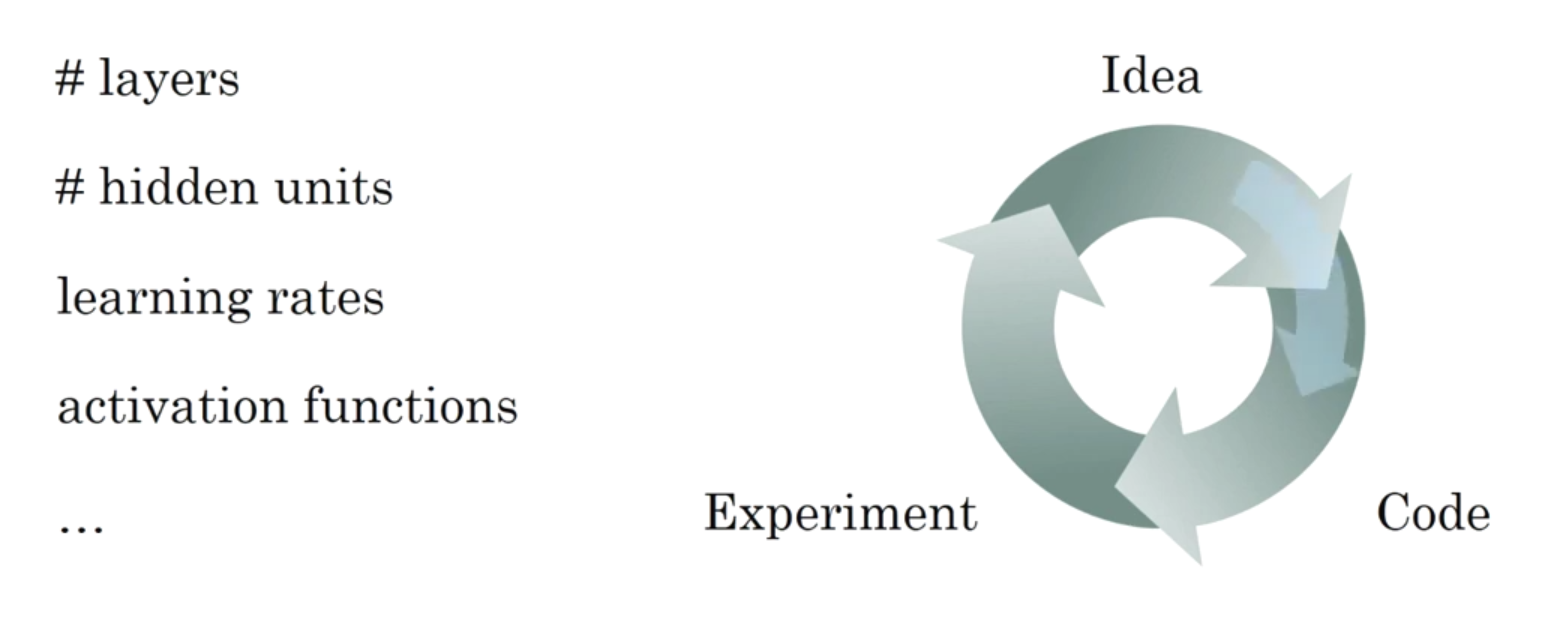
\includegraphics[scale=0.2]{images/iterative.png}
    \centering
\end{figure}

In the previous era of machine learning, it was common to divide all the data and split it according to a 70\%/30\% proportion, and assign them as your train and test sets respectively. Nowadays, however, with the emergence of big data, dev and test sets occcupy a smaller percentage of our data. For example, when we have a dataset with 100000 examples, an 20\% dev set is too big! As a result, the proportions nowadays look like 99.5\%/0.25\%/0.25\%. 

Not having a test set might be okay (only train/dev sets). 


\subsection{Bias/Variance}

The simplest explanation:
\begin{figure}[H]
    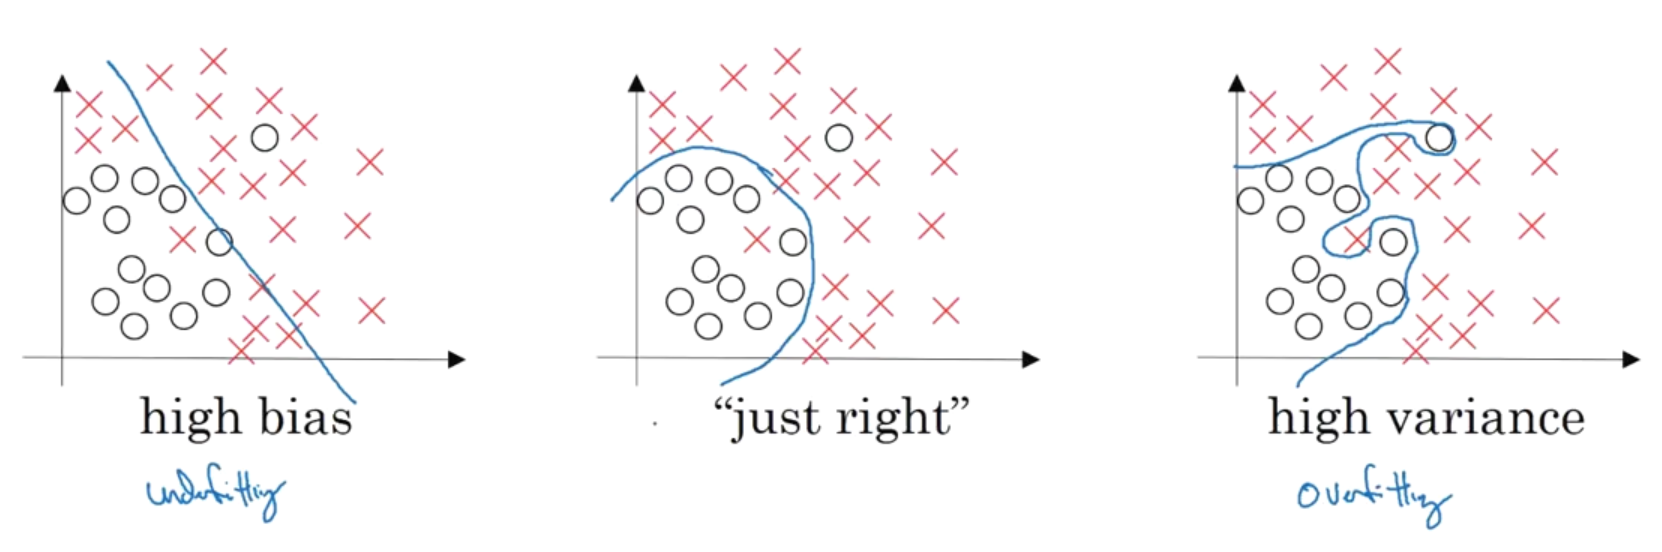
\includegraphics[scale=0.2]{images/biasvariance.png}
    \centering
\end{figure}

Consider another example for a cat classifer. 
\begin{table}[H]
    \begin{tabular}{|c|c|c|c|c|}
    \hline
                & High Variance & High Bias & \begin{tabular}[c]{@{}c@{}}High Bias\\ High Variance\end{tabular} & \begin{tabular}[c]{@{}c@{}}Low Bias\\ Low Variance\end{tabular} \\ \hline
    Train Error & 1\%           & 15\%      & 15\%                                                              & 0.5\%                                                           \\ \hline
    Test Error  & 11\%          & 16\%      & 30\%                                                              & 1.5\%                                                           \\ \hline
    \end{tabular}
\end{table}

The following classifier has both high bias and high variance. High bias because it is a mostly linear classifier, and it mostly underfits; high variance because in some occasions it shows overfitting behavior. 

\begin{figure}[H]
    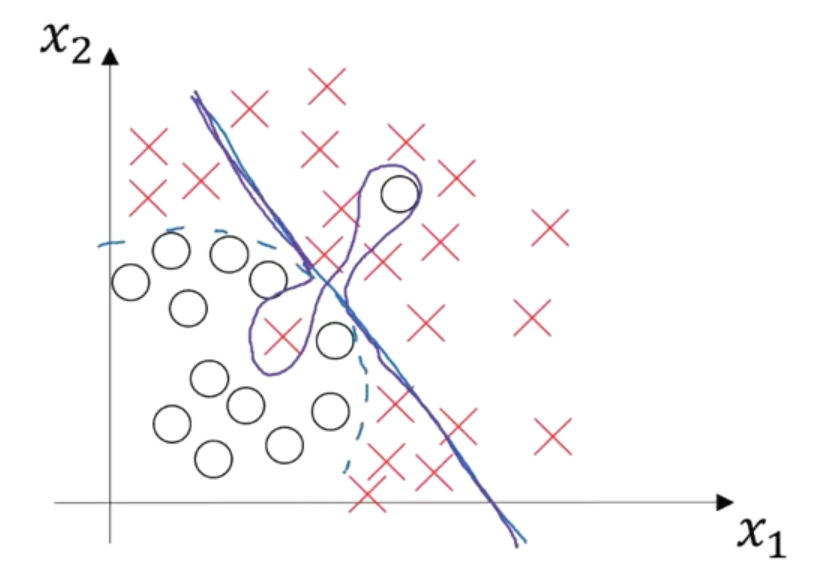
\includegraphics[scale=0.2]{images/highbv.png}
    \centering
\end{figure}

\subsection{Basic Recipe for Machine Learning}
\begin{figure}[H]
    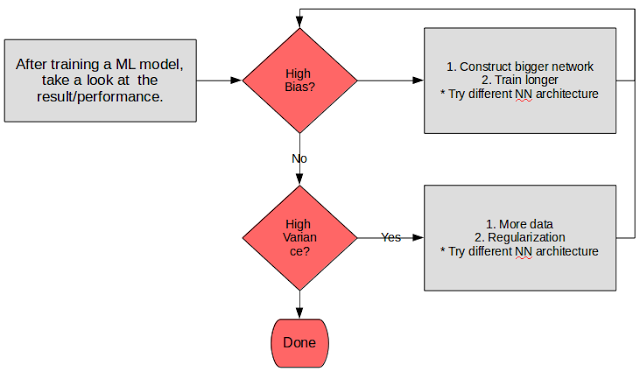
\includegraphics[scale=0.7]{images/recipe.png}
    \centering
\end{figure}

\subsection{Regularization}
If you suspect that your neural network has a high variance problem, meaning that it overfits your data, regularization is one of the first things you should try. The other option is to get more training data, but it is not always viable. 

Remember that in logistic regression, we were trying to minimize $J(w, b)$. Now we add the regularization term to the previous $J$.

$$
J(w, b) = \frac{1}{m}\sum_{i=1}^{m}{L(\yhat^{(i)}, y^{(i)})}+ \frac{\lambda}{2m} \norm{w}_2^{2}
$$ 

It's called $L_2$ regularization because it uses $L_2$ norm, which is: 

$$
\norm{w}_2^2 = \sum_{j=1}^{n_x} w_j^2 = w^T w
$$

It is also possible that we use $L_1$ regularization with the regularization term: 

$$
\frac{\lambda}{2m}\sum_{j=1}^{n_x} |w| = \frac{\lambda}{2m}\norm{w}_1
$$


Note that also a regularization term for bias is possible, but since $b$ is not as high-dimentional as $w$, its regularization term, which is equal to $\frac{\lambda}{m}b^2$, is usually omitted.

In a more complex neural network, though, a more generalized equation will be like this: 

$$
J(W\lay{1}, b\lay{1}, \dots, W\lay{L}, b\lay{L}) = \frac{1}{m}\sum_{i=1}^{m}{L(\yhat^{(i)}, y^{(i)})} + \frac{\lambda}{2m} \sum_{l=1}^L \norm{W\lay{l}}_F^2
$$

$\norm{W\lay{l}}_F^2$ is called the \emph{Frobenius Norm} of the matrix $W\lay{l}$, and knowing that the shape of $W\lay{l}$ is $(n\lay{l-1}, n\lay{l})$ it's computed like this: 

$$
\norm{W\lay{l}}_F^2 = \sum_{i=1}^{n\lay{l-1}} \sum_{j=1}^{n\lay{l}} \Big(w_{ij}^{[l]}\Big)^2
$$

Regularization is also applied to the gradients (it is called \emph{weight decay}): 
$$
dw\lay{l} = (from\ backprop) + \frac{\lambda}{m}w\lay{l}
$$

\subsection{Why Regularization Reduces Overfitting}
Consider a situation where you have a neural network that overfits your data. Remember the original non-regularized cost function: 

$$
J = \frac{1}{m}\sum_{i=1}^{m} L(\yhat^{(i)}, y^{(i)})
$$

In order to reduce overfitting, we penalized $J$ with a regularization term: 
$$
J = \frac{1}{m}\sum_{i=1}^{m} L(\yhat^{(i)}, y^{(i)}) + \frac{\lambda}{2m}\sum_{l=1}^L \norm{W\lay{l}}_F^2
$$

\textbf{Intuition:} If we set $\lambda$ to be a really big number, our minimization algorithm will seek to set $W\lay{l} = 0$, which essentially means that a lot of hidden units will be zeroed out, which means that their impact will be reduced, and we will end up with a simpler neural network that is closer to the "High Bias" realm than it is to the "High Variance" realm.

\textbf{Another Intuition:} Consider using hyperbolic tangent as the activation function. If we regularize our weights, they will become smaller, and as a result, $z = wx+b$ will be smaller. With smaller $z$s, we will be wandering in the "linear section" of $tanh$, which means that each layer will be \emph{roughly} linear, which leaves our network having higher bias. 

\begin{figure}[H]
    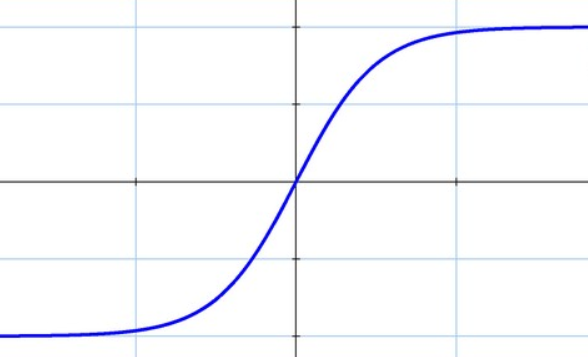
\includegraphics[scale=0.2]{images/tanh.png}
    \centering
\end{figure}

\subsection{Dropout Regularization}
For each node in the network, set some probability for eliminating it. After selecting the to-be-eliminated nodes, remove all the outgoing and incoming links from and to that node, and then do backpropagation on the diminished network.

\begin{figure}[H]
    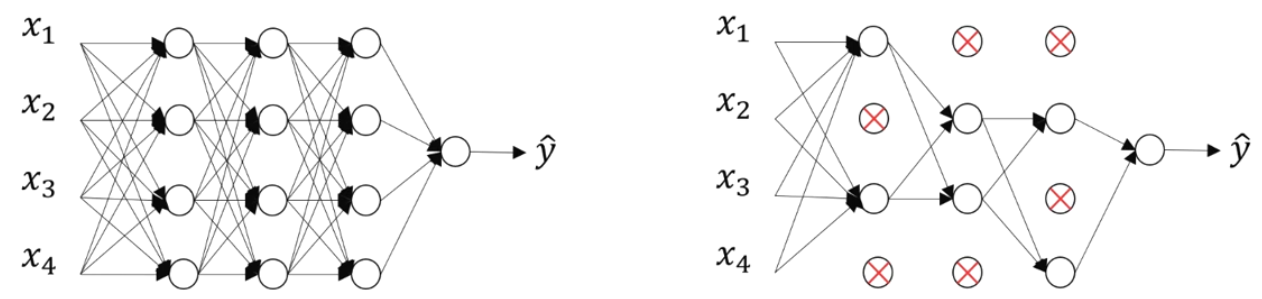
\includegraphics[scale=0.35]{images/dropout.png}
    \centering
\end{figure}

Since you are training a much smaller network \emph{on each example}, you will end up with a regularized network.

\textbf{Dropout Implementation (Inverted Dropout):} Keep in mind that this works for both the vectorized version and the non-vectorized version. Given $l=3$, $keepProb=0.8$: 
$$
d\lay{3} = np.random.rand(a\lay{3}.shape)
$$
$$
a\lay{3} = d\lay{3} \ast a\lay{3}
$$
$$
a\lay{3} /= keepProb
$$

What does the last line do? It keps the expected value of $a\lay{3}$ stable so as to not reduce the value of $z\lay{4} = W\lay{4}a\lay{3}+b\lay{4}$. 

Obviously, there will be no dropout in the test phase, because we do not want to use a random element in our final computation. 

\subsection{Understanding Dropout}
Consider this one particular purple neuron: 

\begin{neuralnetwork}[]
    \newcommand{\x}[2]{$x_#2$}
    \newcommand{\y}[2]{$\hat{y}$}
    \newcommand{\hsecond}[2]{\small $neuron$}
    \inputlayer[count=4, bias=false, title=, text=\x]
    \hiddenlayer[count=1, bias=false, title=, text=\hsecond] \linklayers
\end{neuralnetwork}

As you can see, it relies on 4 features for its value, as a result, using droupout makes the network reluctant to rely heavily on \emph{one} particular feature, employing a more \emph{egalitarian} approach. Droupout has a similar effect to $L_2$ regularization's. 

Another worthy note: It is good practice to keep $keepProp$ variable according to the layer: 

\begin{neuralnetwork}[]
    \newcommand{\x}[2]{$x_#2$}
    \newcommand{\y}[2]{$\hat{y}$}
    \newcommand{\hfirst}[2]{\small $a^{[1]}_#2$}
    \newcommand{\hsecond}[2]{\small $a^{[2]}_#2$}
    \newcommand{\hthird}[2]{\small $a^{[3]}_#2$}
    \newcommand{\hfourth}[2]{\small $a^{[4]}_#2$}

    \inputlayer[count=3, bias=false, title=, text=\x]
    \hiddenlayer[count=7, bias=false, title=, text=\hfirst] \linklayers
    \hiddenlayer[count=7, bias=false, title=, text=\hsecond] \linklayers
    \hiddenlayer[count=3, bias=false, title=, text=\hthird] \linklayers
    \hiddenlayer[count=2, bias=false, title=, text=\hfourth] \linklayers
    \outputlayer[count=1, title=, text=\y] \linklayers
\end{neuralnetwork}


You might choose to use a lower $keepProb$ for layers that have more parameters, because you are more worried about their overfitting ($l=2$ for example). 

\subsection{Other Regularization Methods}
\textbf{Data Augmentation:} Rotating, flipping, distorting and scaling train data images, for example. 

\textbf{Early Stopping:} 
\begin{figure}[H]
    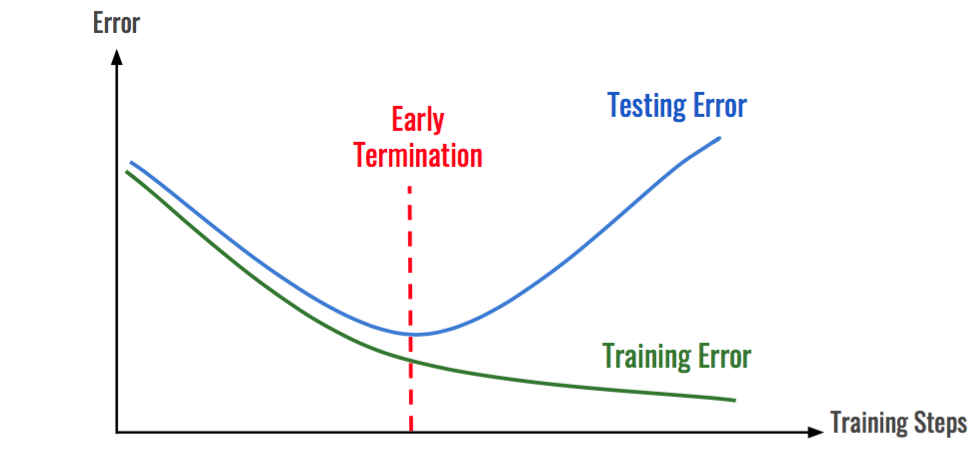
\includegraphics[scale=0.35]{images/earlystop.png}
    \centering
\end{figure}

It does have a downside though, according to the \emph{orthogonalization} principle, we want to worry about one thing at a time. So worrying about the minimization of $J$, and worrying about not overfitting should be handled separately. Early stopping prevents us from doing that. 

\subsection{Normalizing Inputs}

\begin{enumerate}
    \item \textbf{Subtract Mean:}
    $$
    \mu = \frac{1}{m}\sum_{i=1}^{m} X^{(i)}
    $$
    $$
    X^{(i)} = X^{(i)} - \mu\ \ \ \ \ \ \ \forall\ 1 \leq i \leq m
    $$
    \item \textbf{Normalize Variance:}
    $$
    \sigma^2 = \frac{1}{m}\sum_{i=1}^{m} X^{(i)}\ast\ast\ 2
    $$
    $$
    X^{(i)} = X^{(i)} / \sigma^2\ \ \ \ \ \ \ \forall\ 1 \leq i \leq m
    $$
\end{enumerate}

\textbf{Important:} Use the same $\mu, \sigma^2$ to normalize your test set. DO NOT normalize train/dev/test sets with different values of $\mu, \sigma^2$.

\begin{figure}[H]
    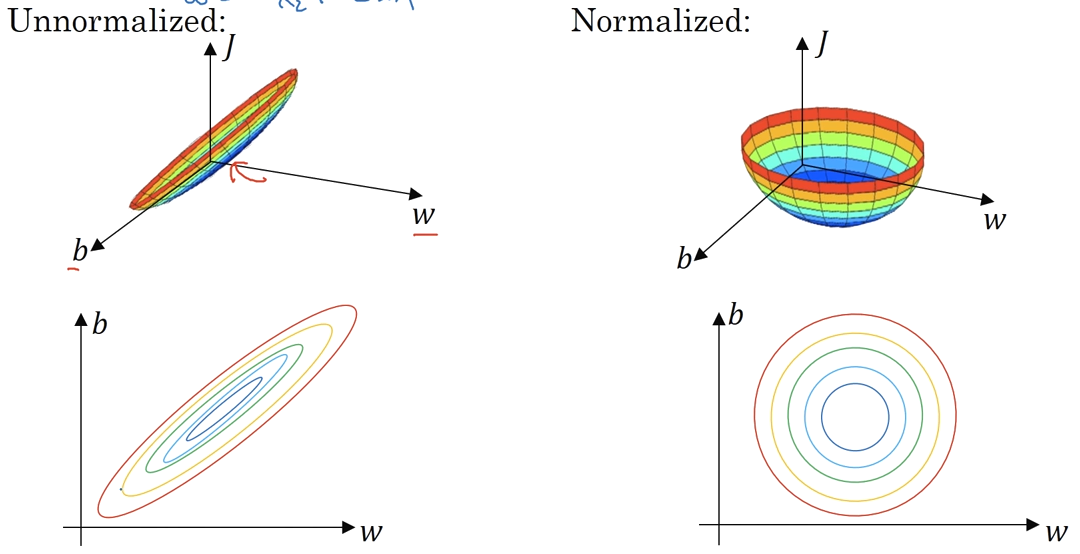
\includegraphics[scale=0.35]{images/normalize.png}
    \centering
\end{figure}

\subsection{Exploding/Vanishing Gradients}
Consider the following deep network, where $g\lay{l}(z)=z, b\lay{l}=0$ in all layers: 

\begin{neuralnetwork}[]
    \newcommand{\x}[2]{$x_#2$}
    \newcommand{\y}[2]{$\hat{y}$}
    \newcommand{\hfirst}[2]{\small $\ $}
    \newcommand{\hsecond}[2]{\small $\ $}
    \newcommand{\hthird}[2]{\small $\ $}
    \newcommand{\hfourth}[2]{\small $\ $}

    \inputlayer[count=2, bias=false, title=, text=\x]
    \hiddenlayer[count=2, bias=false, title=, text=\hfirst] \linklayers
    \hiddenlayer[count=2, bias=false, title=, text=\hsecond] \linklayers
    \hiddenlayer[count=2, bias=false, title=, text=\hthird] \linklayers
    \hiddenlayer[count=2, bias=false, title=, text=\hfourth] \linklayers
    \hiddenlayer[count=2, bias=false, title=, text=\hfourth] \linklayers
    \outputlayer[count=1, title=, text=\y] \linklayers
\end{neuralnetwork}

$$
\yhat = W\lay{L}W\lay{L-1}\dots W\lay{2}W\lay{1}X 
$$

If we have either of the scenarios below, the final $\yhat$ will be either exponentially big or small, making it very difficult to train the network. 

$$
W\lay{l} = \begin{bmatrix}
    1.5 & 0\\
    0 & 1.5
\end{bmatrix} \Rightarrow \yhat = W\lay{L} (1.5)^{L-1} X
$$


$$
W\lay{l} = \begin{bmatrix}
    0.5 & 0\\
    0 & 0.5
\end{bmatrix} \Rightarrow \yhat = W\lay{L} (0.5)^{L-1} X
$$


There is a \emph{partial} solution to this problem, which is careful initialization of the weights. 

\subsection{Weight Initialization in a Deep Network}
Consider this single neuron example, $b=0$: 

\begin{neuralnetwork}[]
    \newcommand{\x}[2]{$x_#2$}
    \newcommand{\y}[2]{$\hat{y}$}
    \newcommand{\hsecond}[2]{\small $z\Big|a$}
    \inputlayer[count=4, bias=false, title=, text=\x]
    \hiddenlayer[count=1, bias=false, title=, text=\hsecond] \linklayers
\end{neuralnetwork}

$$
z = w_1 x_1 + \dots + w_n x_n
$$

Now we don't want $z$ to become too big or too small, so with larger $n$, we want smaller $w_i$s. One solution is to set $Variance(w_i)=\frac{1}{n}$.
$$
w\lay{l} = np.random.randn(shape) \ast np.sqrt(\frac{1}{n\lay{l-1}})
$$

(For ReLU activation functions, $Variance(w_i)=\frac{2}{n\lay{l-1}}$ works better)

(For $tanh$ activation function, $Variance(w_i)=\sqrt{\frac{1}{n\lay{l-1}}}$ and $Variance(w_i)=\sqrt{\frac{2}{n\lay{l-1}+n\lay{n}}}$ work better)

\subsection{Numerical Approximation of Gradients}
$$
g(\theta) \approx \frac{f(\theta + \epsilon) - f(\theta + \epsilon)}{2\epsilon}
$$

\subsection{Gradient Checking}
To verify your backprop implementation is correct. 
\begin{itemize}
    \item Take all your parameters, $W\lay{1}, b\lay{1}, \dots, W\lay{L}, b\lay{L}$, and reshape them into a big vector $\theta$. 
    \item Take all your gradients, $dW\lay{1}, db\lay{1}, \dots, dW\lay{L}, db\lay{L}$, and reshape them into a big vector $d\theta$. 
    \item Now the question is: Is $d\theta$ the gradient of $J(\theta)$?
\end{itemize}

Here's how it's done: 
\begin{itemize}
    \item For each $i$: 
    $$d\theta_{approx}[i]=\frac{J(\theta_1, \theta_2, \dots, \theta_i+\epsilon, \dots) - J(\theta_1, \theta_2, \dots, \theta_i-\epsilon, \dots)}{2\epsilon}$$ 
    $$\approx d\theta[i] = \frac{\partial J}{\partial \theta_i}$$
    \item Now that you have the two vectors $d\theta$ and $d\theta_{approx}$, compute this (the denominator is just a normalizer): 
    $$
    \frac{\norm{d\theta_{approx} - d\theta}_2}{\norm{d\theta_{approx}}_2 + \norm{d\theta}_2}, \epsilon = 10^{-7}
    $$
    \item If the result is $10^{-7}$ or smaller, your gradient is very likely to be working properly. However, you need to double check if the value is too big. 
\end{itemize}